\section{Passage de IPv4 à IPv6}

\subsection{Raison du passage de IPv4 à IPv6}
%\subsubsection{Problème posé par IPv4}


//Pénrurie, adressage privé/publique compliqué
% Il se trouve que apparement il y a des problemes de
% penurie d'adresses meme dans certaines reseau prive`
% http://blog.erratasec.com/2013/12/dod-address-space-its-not-conspiracy.html#.WAf_d7Wf21F

\subsection{Problèmes posés par IPv4}
L'IPv4 a été développé dans les années 70-début des années 80, donc il y a 30-40 ans.
Lors de son développement personne n'a cru qu'internet serait un jour utilisé comme il l'est 
aujourd'hui. N'ayant pas été développé pour l'utilisation que nous en faisons, l'IPv4 présente 
plusieurs problèmes auxquels ont été trouvé des solutions définitives ou provisoires.

\subsubsection{Épuisement des adresses IPv4}

Personne n'aurait imaginé il y a 40 ans qu'il y aurait un jour autant d'interfaces qui se connectent à 
Internet. On pensait que seul les militaires et les scientifiques utiliseront 
internet et qu'un espace d'adressage sur 32 bits serait largement suffisant. 
De plus, les plages d'adresses étaient distribuées généreusement au début. 
Cela veut dire que l'on attribuait des adresses permettant la création de réseaux 
avec un nombre d'interfaces pouvant se connecter largement au-dessus de ce qui était 
nécessaire.
Cependant, avec la croissance du nombre d'utilisateurs et des équipements connectés, 
la plage d'adresses IPv4 disponible a diminué progressivement. C'est en février 2011 
que la réserve de bloc d'adresses publiques libres IPv4 de l'IANA (Internet Assigned 
Numbers Authority) est arrivée à épuisement. En plus de cela la répartition très inégale des adresses est également constatée. 
La zone américaine est très favorisée (environ 74\%) par rapport à l'Europe (environ 17\%) et l'Asie (environ 9\%).


\subsection{Sécurité}
Même s'il existe beaucoup de protocoles pour assurer la sécurité sous IPv4, il y en a 
beaucoup qui ne sont pas standardisé. L'IPv6 a standardisé et rendu obligatoire des 
technologies dont certaines étaient auparavant utilisées dans IPv4. 

\subsection{Performances}
Sous IPv4, la taille des paquets est petite. De plus, chaque routeur ne supporte pas la même taille
de paquet. Il arrive donc fréquemment que les paquets doivent être fragmentés. Dans Ipv4, ce sont les 
routeurs et autre équipements intermédiaires qui font ce travail. Cela peut amener à
des diminutions de performances lorsqu'un routeur a à fragmenter beaucoup de paquets ou
lorsque sa puissance de calcul est limitée. 
\\
De plus, sous IPv4, les routeurs vérifient l'intégrité des paquets lors du transit, ce qui nécessite 
des ressources pour vérifier à chaque fois le checksum, qui changeait à chaque saut à cause
de la décrémentation de Time To Live.
\\
Il existe également un défaut de performances pour les équipements mobiles comme les téléphones 
portables. Ceux-ci changent en effet souvent de réseau et ils changent, à cause de 
l'utilisation du NAT ou d'un changement de connexion 4G à une connexion, souvent d'adresse IP. 
\\


\subsection{Solutions pour l'épuisement des adresses IPv4}

Afin de résoudre ce problème, plusieurs techniques ont été proposées:
\begin{itemize}
\item La première a été le changement de technique d'adressage. On est passé de la
technique de classe d'adressage IP à la technique \textbf{Classless Inter-Domain
Routing}. Ceci a permit une meilleure efficacité dans la distribution des
adresses IP grâce à la création de réseau de tailles intermédiaire. En effet,
avant on ne disposait que de réseau de 3 tailles différentes et l'on attribuait
souvent des adresses permettant des réseaux bien plus grand que nécessaire.

\item Les politiques d'assignement d'adresses ont également été rendues plus stricte
afin de mieux tenir compte des besoin réels des demandeurs d'adresses IP.

\item Des blocs autrefois réservé comme 14.0.0.0 ont également été distribués.

\item Sur base de volontarisme, des blocs autrefois attribués généreusement ou alors
des IP non utilisées ont été récupérées.

\item Finalement, il a été remarqué qu'il n'était pas nécessaire que chaque interface
a sa propre adresse IP publique et le protocole NAT a été développé afin de regrouper
plusieurs interfaces sous une même adresse IP. Ce protocole est de plus en plus
utilisé dans IPv4 depuis la fin des années 90. Le fonctionnement du NAT sera explicité
plus loin.
\end{itemize}


\subsubsection{CIDR(Classless Inter-Domain Routing)}
Nous avons vu le fonctionnement du CIDR dans la partie fonctionnement. Pour rappel, le
CIDR a été développé en 1993 dans le but de diminuer la taille des tables de routage. Pour 
cela le concept de classe d'adresse a été abandonné et a été remplacé par une agrégation de 
plusieurs entrées dans une table de routage par une seule entrée.
Avec ce nouveau concept il a été possible de diviser une adresse IP plus finement. Cela veut 
dire qu'il est maintenant possible de donner des plages d'adresse ayant des préfixes allant 
de 0 à 31. Il est donc possible de créer 31 sortes de réseaux de taille différente. Il y a 
donc, d'une part, moins de gaspillage d'adresse IP, et d'autre part, il y en a plus qui sont disponibles.

\subsubsection{Traduction d'adresse réseau (Network Adress Translation}
Comme vu au-dessus, au fur et à mesure que l'IPv4 s'est répandu, il y a eu un manque
d'espace d'adressage. Afin de limiter le nombre d'adresse IP publiques nécessaires
à un réseau, le NAT a été développé.

\subsubsection{Fonctionnement du NAT dynamique (Network Adress Translation)}
Le NAT est une technique utilisée au niveau du routeur. Le principe du NAT est
que le routeur fait correspondre à une adresse IP une autre adresse IP en
changeant l'adresse IP dans les headers des paquets IP. Cette technique permet
d'échanger des paquets entre 2 domaines d'adresses. En général cette technique
est utilisée pour avoir une même adresse IP pour tout un réseau comme un 
intranet ou encore un réseau domestique. Dans ce réseau, toutes les interfaces
- même le routeur - auront une adresse privée. Le routeur dispose en plus de
cela de une ou plusieurs adresses publiques avec lesquelles il est connecté à
internet. Une adresse privée est une adresse qui est utilisée à l'intérieur
d'un réseau local. Dans un réseau local, les adresses utilisées sont locales et donc
indépendantes de tout réseau externe. Cela veut dire qu'elles n'ont aucune
signification en dehors du réseau local et qu'elles ne sont donc utilisées qu'à
l'intérieur de celui-ci. Les adresses privées peuvent être choisies parmi les
suivantes: 10.0.0.0/8, 172.16.0.0/12 ou 192.168.0.0/16.
\smallbreak
Lorsqu'une interface envoie un paquet vers l'extérieur du réseau, le routeur
effectue plusieurs changements. Il traduit d'abord l'adresse privée en adresse
publique et la met dans l'en-tête du paquet. Puis il change tous les checksums
qui tiennent compte de l'adresse IP. Enfin, il garde en mémoire dans une table,
 appelée table NAT la correspondance entre adresse privée/adresse publique et le
protocole utilisé.
\newline
Cela n'est cependant pas suffisant. En effet, lorsqu'un paquet arrivera de
l'extérieur du réseau, et si toutes les interfaces utilisent la même adresse
publique sans distinction supplémentaire, le routeur ne saura pas à quelle
interface envoyer le paquet et il sera donc perdu.

Une solution à ce problème existe pour les protocoles utilisant les ports comme
TCP et UDP. Le routeur ajoute des informations supplémentaires dans la table qui
sont le port source et destination d'où viennent le paquet. Les ports, qui sont implémentés dans
la couche transport (couche 4), sont des sortes de "portes" qui permettent de
communiquer avec un système d'exploitation. Le numéro de port est un numéro
choisit aléatoirement entre 1024 et 65535 pour le client. Les ports 0 à 1023 étant réservés
pour les serveurs qui "écoutent" pour des connexions entrantes.
\newline
Pour illustrer le fonctionnement du NAT imaginons qu'une interface A dont l'ip
est 192.168.0.1 veut envoyer un paquet TCP à l'interface B d'ip 217.70.184.38.
Le port source est le port 10277 et le port destination est le port 80. Le
routeur, qui est une box, a l'adresse IP  82.240.25.50.

L'interface A envoie le paquet:
\includegraphics{./pics/PaquetAR.eps}

La box effectue un changement de l'adresse et envoie le paquet:
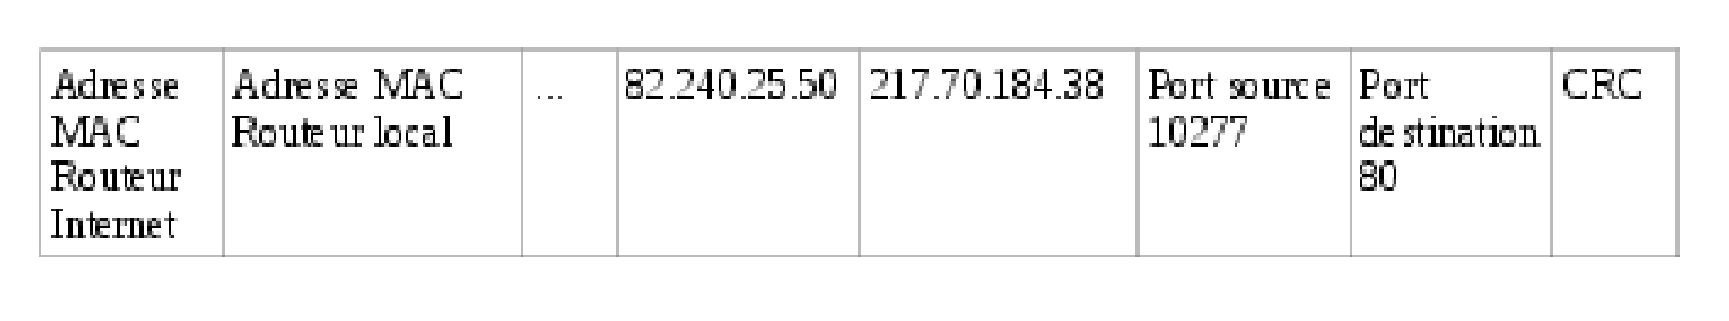
\includegraphics{./pics/PaquetRB.eps}
L'interface B répondra en envoyant le paquet:
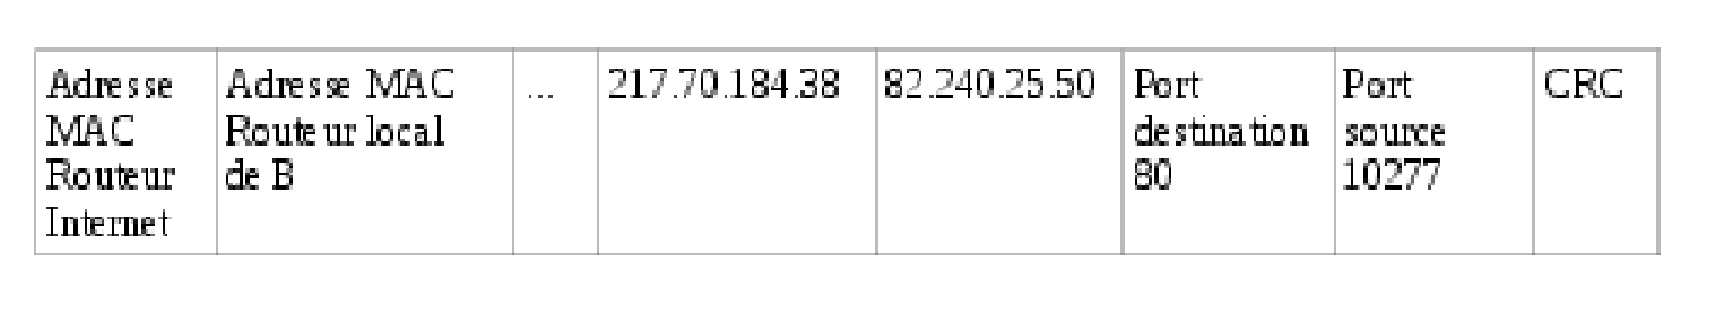
\includegraphics{./pics/PaquetBR.eps}
\smallbreak
Finalement, la table NAT ressemblera à ceci:

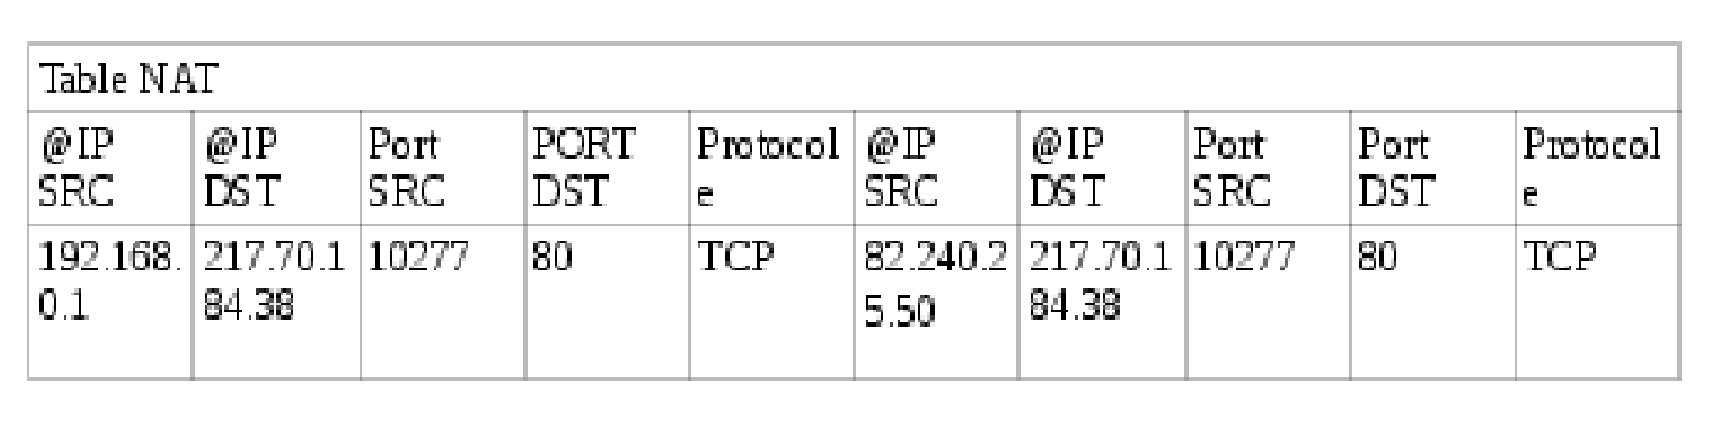
\includegraphics{./pics/TableNAT1.eps}

Lorsque la box reçoit ce paquet, elle voit que le port de destination est le
port 10277. Elle cherche ensuite le port correspondant dans sa table NAT.
Lorsqu'elle le trouve elle effectue les changements nécessaire sur le paquet et
transmet le paquet à l'interface A.
\newline
Mais même si cette solution fonctionne la plupart du temps, la probabilité est
faible, mais existe, que 2 interfaces envoient des paquet sur les même port. Par exemple,
lorsque 2 interfaces envoient des paquets à un serveur HTTP, elles utilisent le port 80. 
C'est pour éviter cela que la box change le port source lorsqu'elle reçoit un paquet de
l'interface A. Ainsi on s'assure que aucun port n'est utilisé plusieurs fois.
On obtient donc des tables de NAT comme dans l'exemple ci dessous:
\newline
On reprend les mêmes informations qu'avant. On a donc une interface A dont l'ip
est 192.168.0.1 veut envoyer un paquet TCP à l'interface B d'ip 217.70.184.38.
Le port source est le port 10277 et le port destination est le port 80. Le
routeur a l'adresse IP  82.240.25.50.
On y ajoute une interface C, sur le même réseau que A et qui veut également
envoyer un paquet TCP à la même adresse avec le même port source. L'IP de C
sera 192.168.1.2.
On obtient la table:
\includegraphics{./pics/TableNAT2.eps}

Enfin, pour éviter de saturer les ports utilisés il est nécessaire de recycler
 ceux qui ne sont plus utilisés. Lorsqu'on utilise un protocole comme UDP le
routeur n'a aucune possibilité de savoir si le transfert est terminé. Lorsqu'on
utilise une connexion TCP entre A et B, des messages de fin de session sont
envoyés par A et B lors de la fin du transfert. Lorsque la transmission est
finit, A envoie un message FIN à B qui lui répond par un message ACK et vice
versa. Mais ces messages ne sont pas utilisables pour reconnaître la fin de
connexion car lors de la réception de ce message il est toujours possible qu'un
paquet ai du être retransmit. Ainsi, on utilise un compteur de temps qui est
associé à chaque paire adresse publique/adresse privée. Lorsqu'il n'y a pas de
trafic entre une adresse privée et l'extérieur durant une durée fixée, le port
qui lui est associée peut être réutilisé pour une autre adresse privée.

\subsubsection{Différents types de NAT}

Il existe différents types de NAT:
\begin{itemize}
\item Le NAT dynamique PAT (Port Address Translation du port source). Ici les
adresses externes sont indifférentes. C'est le mécanisme qui utilise le port forwarding.
\item Masquerading où il n'y a qu'une adresse IP, celle du routeur, qui est
utilisée comme adresse IP externe.
\item NAT pool de source. Ici la première connexion privée prend la première
adresse ip externe, la deuxième prend la deuxième ip externe, etc.
\item NAT pool de destination. Elle permet de répartir la charge entre plusieurs
serveurs.
\end{itemize}


\subsubsection{Redirection de port(Port forwarding)}

Le NAT dynamique apporte cependant un grand problème. Lorsqu'une interface
extérieur veut se connecter à une interface dans le réseau, elle ne dispose
d'aucune autre information que l'adresse IP publique. Si elle envoie alors un
paquet à cette adresse, le routeur qui le réceptionnera ne saura pas quoi en
faire car il ne sait pas à quelle interface le paquet est destiné et le paquet sera
donc perdu. Il n'est donc pas possible, pour une machine externe au réseau local, d'établir 
une connexion avec une interface connectée au réseau local.

On a réussi à pallier à ce problème grâce à la redirection de port (port 
forwarding). 

Le principe du port forwarding est de rediriger tout paquet qui arrive sur un
port du routeur vers le port d'une interface locale.
Par exemple, prenons un routeur qui a comme IP externe 82.240.25.50.
Nous le réglons de façon qu'il redirige tout paquet arrivant sur son port 80
vers une interface locale A d'adresse locale 192.168.1.1.
Imaginons qu'une interface sur le réseau essaie de se connecter à cette adresse
 IP au port 80.
Lorsque le routeur reçoit le paquet il va le transmettre à l'interface A comme
dans le schéma ci-dessous:

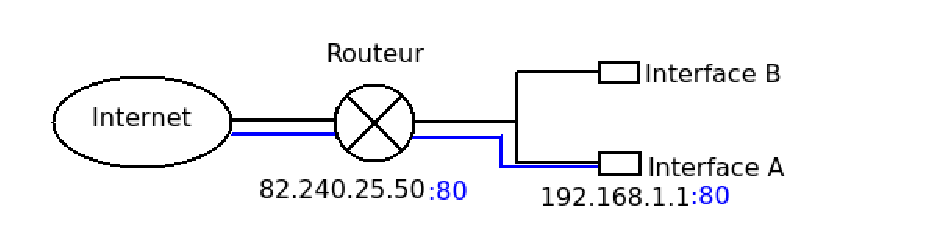
\includegraphics{./pics/port_forwarding.eps}

Il est possible de faire du port forwarding sur plusieurs port et vers des
interfaces différentes simultanément.

\subsubsection{NAT statique}
Le NAT statique est l'attribution d'une adresse IP externe à une adresse IP 
privée. Grâce à cette méthode une interface sur un réseau privé peut avoir une
IP publique à elle seule. Pour faire une traduction d'adresse statique il faut la configurer
manuellement dans la table de routage du routeur. Cette traduction restera dans
la table jusqu'à ce qu'elle soit supprimée. La traduction d'adresse statique
est le plus souvent utilisée pour interconnecter deux réseaux avec des
adressages différents.

\subsubsection{NAT et sécurité}

Même si ça n'a pas été le but de la traduction d'adresses, un des effets
secondaires du NAT a été d'apporter de la sécurité. En effet, auparavant, une
interface pouvait se connecter à n'importe quel port sur une machine du réseau,
à condition que ce port soit ouvert. Certains systèmes comme Windows ouvrent des ports
par défaut pour "écouter" le réseau. Avec la traduction d'adresse, il n'est pas
possible d'atteindre n'importe quel port d'une interface. Il est uniquement
possible d'atteindre un port lorsqu'une connexion a été établit avec ce port
spécifique ou si le routeur cible a configuré l'interface cible comme interface
par défaut pour ce port.


Cependant même toutes ces solutions n'ont pas suffit pour +++

\subsection{Améliorations apportés par IPv6}

De nombreuses améliorations ont été apportées par IPv6, qui est une refont d'IPv4, afin de répondre à des besoins existants. Le fonctionnement de l'IPv6 reste cependant très similaire à celui d'IPv4 et 
les protocoles TCP et UDP sont quasiment inchangés.
l'IPv6 a été finalisée en 1998 et a été publiée dans la RFC2460. Lorsque l'IPv6 a été développée, 
l'utilisation et la direction que prenait internet était donc déjà claire. 

\subsubsection{Espaces d'adressage}
Dans l'IPv6, les adresses sont codées sur 128 bits, soit 16 octets. Cela permet d'avoir 
environ quatre milliards de fois plus d'adresse qu'en IPv4. Tous les soucis d'espace d'adressage sont donc levés. Il n'est donc plus nécessaire d'utiliser des technologies comme les traductions d'adresses
(NAT) afin d'économiser des adresses publiques. Le fonctionnement en est donc rendu plus simple car 
chaque interface peut avoir une IP publique et il n'y a pas de problème pour atteindre une interface sur le réseau.
\subsubsection{Sécurité}
Comme dit précédemment, même s'il existait des protocoles de sécurité pour IPv4, 
ces derniers ne faisaient pas partie intégrante du protocole.
Dans IPv6, des mesures de sécurités ont été directement intégrées au protocole.
Par exemple, le chiffrement et la vérification de l'intégrité utilisés dans les réseaux privés 
(VPN, Virtual Private Network) est une composante standard pour IPv6 alors qu'elle était 
facultative pour IPv4. Grâce à cet ajout, certaines attaques informatiques comme l'attaque de 
l'homme du milieu, qui consiste à se faire passer pour quelqu'un d'autre et d'intercepter 
le trafic, seront rendues plus difficiles.
\\
De plus, IPv6 apporte une résolution de noms plus sécurisée grâce au protocole Secure Neighbor
Discovery (SEND) qui permet de confirmer qu'un hôte est bien celui qu'il prétend être. Ainsi, la redirection de trafic est rendue plus difficile.
\\
Enfin, une sécurité est intégrée dans l'IPv6. Cette sécurité est IPsec. Celle-ci était optionnelle 
dans IPv4 et a été rendue obligatoire en IPv6.
\subsubsection{Performances}

Le système de routage est beaucoup plus efficace. En effet, les paquets IPv6 ne sont plus
fragmentés par les routeurs mais par l'interface qui envoie le paquet. Lorsqu'une interface
veut envoyer un paquet, elle envoie d'abord un message ICMPv6 pour déterminer le MTU qui est 
la taille des paquets qui seront envoyés.
\\
L'élimination du NAT permet de supprimer un niveau intermédiaire et les problèmes liées à celui-ci
 comme l'accessibilité d'une interface en dehors du réseau.
\\	
L'amélioration de la structure d'en-tête permet d'alléger le traitement. La
plupart des champs dans l'en-tête IPv4 étaient facultatifs et utilisés
fréquemment. IPv6 élimine ces champs (les options sont traitées différemment).
